\documentclass[10pt]{beamer}
\usetheme[
%%% option passed to the outer theme
%    progressstyle=fixedCircCnt,   % fixedCircCnt, movingCircCnt (moving is deault)
  ]{Feather}
  
% If you want to change the colors of the various elements in the theme, edit and uncomment the following lines

% Change the bar colors:
\setbeamercolor{Feather}{fg=black!20,bg=black}

% Change the color of the structural elements:
\setbeamercolor{structure}{fg=black}

% Change the frame title text color:
%\setbeamercolor{frametitle}{fg=blue}

% Change the normal text color background:
%\setbeamercolor{normal text}{fg=black,bg=gray!10}

%-------------------------------------------------------
% INCLUDE PACKAGES
%-------------------------------------------------------

\usepackage[utf8]{inputenc}
\usepackage[polish]{babel}
\usepackage{polski}
\usepackage[T1]{fontenc}
\usepackage{helvet}
\usepackage{booktabs}
\usepackage{array}
\usepackage{setspace}
\usepackage{graphicx}
\usepackage{caption}
\usepackage{soul}


%-------------------------------------------------------
% DEFFINING AND REDEFINING COMMANDS
%-------------------------------------------------------
\DeclareCaptionLabelSeparator{kropka}{. }
\setbeamertemplate{caption}[numbered]
\captionsetup[figure]{labelformat=simple, labelsep=kropka}
\captionsetup[table]{labelformat=simple, labelsep=kropka}
\addto\captionspolish{\renewcommand{\tablename}{Tabela}}

\newcolumntype{k}[1]{>{\centering\arraybackslash}m{#1}}

% colored hyperlinks
\newcommand{\chref}[2]{
  \href{#1}{{\usebeamercolor[bg]{Feather}#2}}
}

%-------------------------------------------------------
% INFORMATION IN THE TITLE PAGE
%-------------------------------------------------------

\title[Zastosowanie algorytmów ewolucyjnych do wyznaczania przybliżonych reduktów] % [] is optional - is placed on the bottom of the sidebar on every slide
{ % is placed on the title page
      \textbf{Zastosowanie algorytmów ewolucyjnych do~wyznaczania przybliżonych reduktów}
}

\author[Jan Gromko]
{
	\textbf{Dyplomant: Jan Gromko}\\
	\textbf{Promotor: prof. dr hab. Jarosław Stepaniuk}
}

\institute[WI PB]
{
      Wydział Informatyki Politechniki Białostockiej
}

\date{19 kwietnia 2017 r.}


\begin{document}


{\1% wybór pliku na tło
\begin{frame}[plain,noframenumbering]
\begin{spacing}{1.5}
  \titlepage
\end{spacing}
\end{frame}}


\begin{frame}{Plan prezentacji}{}
\tableofcontents
\end{frame}


\section{Redukcja}

\subsection{Istota problemu redukcji}
\begin{frame}{Redukcja}
\begin{spacing}{1.5}
\textbf{Czy można zredukować zbiór pod~względem atrybutów w~ten~sposób, by~zachowana była rozróżnialność elementów z~oryginalnego zbioru?}
\end{spacing}
\end{frame}

\begin{frame}
\frametitle{Redukcja}
\begin{spacing}{1.5}
\begin{block}{Zbiór niezależny}
Zbiór atrybutów $B_{1} \subset A$ jest \textit{niezależny} w danym systemie informacyjnym, jeśli dla każdego $B_{2} \subset B_{1}$ zachodzi $IND(B_{1}) \neq IND(B_{2})$.
\end{block}

\begin{block}{Redukt}
\textit{Reduktem} zbioru atrybutów $B_{1} \subseteq A$ nazywamy każdy niezależny zbiór $B_{2} \subseteq B_{1}$, dla którego $IND(B_{1}) = IND(B_{2})$, przy czym $B_{2}$ powinien być 
jak najmniej liczny. Może istnieć wiele reduktów.
\end{block}
\end{spacing}
\end{frame}


\begin{frame}{Przykładowy zbiór}
\begin{center}
\begin{table}
\begin{tabular}{|k{1.2cm}|k{1.8cm}|k{1.8cm}|k{2.2cm}|k{1.4cm}|@{}m{0pt}@{}}
\hline
\textit{Pacjent} & \textit{Ból głowy} & \textit{Ból mięśni} & \textit{Temperatura} &  \textit{Grypa} &\\[1ex]
\hline
1 & nie & tak & podwyższona & tak &\\[1ex]
2 & tak & nie & podwyższona & tak &\\[1ex]
3 & tak & tak & wysoka & tak &\\[1ex]
4 & nie & tak & normalna & nie &\\[1ex]
5 & tak & nie & podwyższona & nie &\\[1ex]
6 & nie & nie & wysoka & tak &\\[1ex]
\hline
\end{tabular}
\caption{Tablica decyzyjna przykładowego zbioru.}
\end{table}
\end{center}
\end{frame}


\begin{frame}{Macierz rozróżnialności}
\renewcommand{\arraystretch}{1}
\begin{center}
\begin{table}
\begin{tabular}{|k{1cm}|k{1cm}|k{1cm}|k{1cm}|k{1cm}|k{1cm}|k{1cm}|@{}m{0pt}@{}}
\hline
& 1 & 2 & 3 & 4 & 5 & 6&\\[1ex]
\hline
1 & $\emptyset$ & -- & -- & -- & -- & -- &\\[1ex]
\hline
2 & $\emptyset$ & $\emptyset$ & -- & -- & -- & -- &\\[1ex]
\hline
3 & $\emptyset$ & $\emptyset$ & $\emptyset$ & -- & -- & -- &\\[1ex]
\hline
4 & t & g, m, t & g, t & $\emptyset$ & -- & -- &\\[1ex]
\hline
5 & g, m & $\emptyset$ & m, t & $\emptyset$ & $\emptyset$ & -- &\\[1ex]
\hline
6 &$\emptyset$ & $\emptyset$ & $\emptyset$ & m, t & g, t & $\emptyset$ &\\[1ex]
\hline
\end{tabular}
\caption{Macierz rozróżnialności.}
\end{table}

\end{center}

\begin{flushleft}
\textit{g} -- ból głowy; 
\textit{m} -- ból mięśni; 
\textit{t} -- temperatura
\end{flushleft}

\end{frame}




\begin{frame}{Macierz rozróżnialności -- redukcja}
\renewcommand{\arraystretch}{1}
\begin{center}
\begin{table}
\begin{tabular}{|k{1cm}|k{1cm}|k{1cm}|k{1cm}|k{1cm}|k{1cm}|k{1cm}|@{}m{0pt}@{}}
\hline
& 1 & 2 & 3 & 4 & 5 & 6 &\\[1ex]
\hline
1 & $\emptyset$ & -- & -- & -- & -- & --&\\[1ex]
\hline
2 & $\emptyset$ & $\emptyset$ & -- & -- & -- & --&\\[1ex]
\hline
3 & $\emptyset$ & $\emptyset$ & $\emptyset$ & -- & -- & --&\\[1ex]
\hline
4 & t & g, t & g, t & $\emptyset$ & -- & --&\\[1ex]
\hline
5 & g & $\emptyset$ & t & $\emptyset$ & $\emptyset$ & --&\\[1ex]
\hline
6 &$\emptyset$ & $\emptyset$ & $\emptyset$ & t & g, t & $\emptyset$&\\[1ex]
\hline
\end{tabular}
\caption{Macierz rozróżnialności po redukcji.}
\end{table}

\end{center}

\end{frame}


\subsection{Prosty algorytm wyznaczania reduktu}

\begin{frame}{Prosty algorytm wyznaczania reduktu}
\begin{spacing}{1.5}
\begin{enumerate}
\item Zliczenie wystąpień atrybutów w macierzy rozróżnialności.
\item Wybór atrybutu występującego najliczniej w macierzy rozróżnialności; dodanie wybranego atrybutu do wynikowego zbioru atrybutów $Red$.
\item Wykreślenie komórek zawierających wybrany atrybut.
\item Jeśli wszystkie komórki zostały wykreślone, wynikiem jest uzyskany zbiór $Red$, w przeciwnym razie powrót do kroku 1.
\end{enumerate}
\end{spacing}
\end{frame}



\begin{frame}{Prosty algorytm redukcji}
\renewcommand{\arraystretch}{1}
\begin{center}
\begin{table}
\begin{tabular}{|k{1cm}|k{1cm}|k{1cm}|k{1cm}|k{1cm}|k{1cm}|k{1cm}|@{}m{0pt}@{}}
\hline
& 1 & 2 & 3 & 4 & 5 & 6&\\[1ex]
\hline
4 & t & g, m, t & g, t & $\emptyset$ & -- & -- &\\[1ex]
\hline
5 & g, m & $\emptyset$ & m, t & $\emptyset$ & $\emptyset$ & -- &\\[1ex]
\hline
6 &$\emptyset$ & $\emptyset$ & $\emptyset$ & m, t & g, t & $\emptyset$ &\\[1ex]
\hline
\end{tabular}
\caption{Fragment macierzy rozróżnialności zawierający istotne dane.}
\end{table}
$\newline$
\begin{spacing}{1.5}
g -- 4~~~~~~~~~~~~~m -- 4~~~~~~~~~~~~~\alert{t -- 6}\\
\end{spacing}
\end{center}
\end{frame}


\begin{frame}{Prosty algorytm redukcji}
\renewcommand{\arraystretch}{1}
\begin{center}
\begin{table}
\begin{tabular}{|k{1cm}|k{1cm}|k{1cm}|k{1cm}|k{1cm}|k{1cm}|k{1cm}|@{}m{0pt}@{}}
\hline
& 1 & 2 & 3 & 4 & 5 & 6&\\[1ex]
\hline
4 & \st{t} & \st{g, m, t} & \st{g, t} & $\emptyset$ & -- & -- &\\[1ex]
\hline
5 & g, m & $\emptyset$ & \st{m, t} & $\emptyset$ & $\emptyset$ & -- &\\[1ex]
\hline
6 &$\emptyset$ & $\emptyset$ & $\emptyset$ & \st{m, t} & \st{g, t} & $\emptyset$ &\\[1ex]
\hline
\end{tabular}
\caption{Fragment macierzy rozróżnialności zawierający istotne dane.}
\end{table}
$\newline$
\begin{spacing}{1.5}
$Red = \lbrace t \rbrace$\\
\alert{g -- 1~~~~~~~~~~~~~m -- 1}
\end{spacing}
\end{center}
\end{frame}


\begin{frame}{Prosty algorytm redukcji}
\renewcommand{\arraystretch}{1}
\begin{center}
\begin{table}
\begin{tabular}{|k{1cm}|k{1cm}|k{1cm}|k{1cm}|k{1cm}|k{1cm}|k{1cm}|@{}m{0pt}@{}}
\hline
& 1 & 2 & 3 & 4 & 5 & 6&\\[1ex]
\hline
4 & \st{t} & \st{g, m, t} & \st{g, t} & $\emptyset$ & -- & -- &\\[1ex]
\hline
5 & \st{g, m} & $\emptyset$ & \st{m, t} & $\emptyset$ & $\emptyset$ & -- &\\[1ex]
\hline
6 &$\emptyset$ & $\emptyset$ & $\emptyset$ & \st{m, t} & \st{g, t} & $\emptyset$ &\\[1ex]
\hline
\end{tabular}
\caption{Fragment macierzy rozróżnialności zawierający istotne dane.}
\end{table}
$\newline$
\begin{spacing}{1.5}
$Red = \lbrace t, g \rbrace \vee Red = \lbrace t, m \rbrace$\\
\end{spacing}
\end{center}
\end{frame}


\begin{frame}{Rdzeń}
\renewcommand{\arraystretch}{1}
\begin{center}
\begin{table}
\begin{tabular}{|k{1cm}|k{1cm}|k{1cm}|k{1cm}|k{1cm}|k{1cm}|k{1cm}|@{}m{0pt}@{}}
\hline
& 1 & 2 & 3 & 4 & 5 & 6&\\[1ex]
\hline
1 & $\emptyset$ & -- & -- & -- & -- & -- &\\[1ex]
\hline
2 & $\emptyset$ & $\emptyset$ & -- & -- & -- & -- &\\[1ex]
\hline
3 & $\emptyset$ & $\emptyset$ & $\emptyset$ & -- & -- & -- &\\[1ex]
\hline
4 & \alert{t} & g, m, t & g, t & $\emptyset$ & -- & -- &\\[1ex]
\hline
5 & g, m & $\emptyset$ & m, t & $\emptyset$ & $\emptyset$ & -- &\\[1ex]
\hline
6 &$\emptyset$ & $\emptyset$ & $\emptyset$ & m, t & g, t & $\emptyset$ &\\[1ex]
\hline
\end{tabular}
\caption{Macierz rozróżnialności oryginalnego zbioru.}
\end{table}
\begin{spacing}{1.5}
$Red = \lbrace \alert{t}, g \rbrace \vee Red = \lbrace \alert{t}, m \rbrace$\\
\end{spacing}
\end{center}
\end{frame}


\begin{frame}{Zbiory przybliżone -- definicje}
\begin{spacing}{1.3}

\begin{block}{Atrybut nieusuwalny}
Atrybut $p\in P_{1}$ jest \textit{nieusuwalny} z $P_{1}$, jeśli dla $P_{2} = P_{1}\setminus\lbrace p\rbrace$ zachodzi $\widetilde{P_{2}} \neq \widetilde{P_{1}}$. W przeciwnym przypadku atrybut $p$ jest \textit{zbędny}.
\end{block}

\begin{block}{Rdzeń}
\textit{Rdzeniem P} nazywa się zbiór wszystkich atrybutów nieusuwalnych\\
ze zbioru P, co zapisywane jest w następujący sposób:
$$CORE(P) = \lbrace p \in P : \widetilde{P'} \neq \widetilde{P}, P'=P\setminus \lbrace p \rbrace\rbrace.$$
\end{block}

\end{spacing}
\end{frame}


\subsection{Problem złożoności dokładnych algorytmów redukcji}
\begin{frame}{Problem złożoności wyznaczania reduktu}
\begin{spacing}{1.5}
Wyznaczanie reduktu w zbiorze przybliżonym jest problemem NP-zupełnym -- nie jest możliwe znalezienie rozwiązania w~czasie~wielomianowym.
\end{spacing}
\end{frame}

\subsection{Alternatywne metody redukcji}
\begin{frame}{Alternatywne metody wyznaczania reduktu}
\begin{spacing}{1.5}
Rozwiązania sprzętowe:\\
\begin{itemize}
\item specjalizowane układy programowalne (FPGA, CPLD).
\end{itemize}

Rozwiązania przybliżone -- wykorzystanie innych metod sztucznej~inteligencji:\\
\begin{itemize}
\item \alert{algorytmy ewolucyjne},
\item algorytmy mrówkowe,
\item inteligencja roju,
\item metody połączone.
\end{itemize}
\end{spacing}
\end{frame}


\section{Propozycje algorytmów genetycznych do wyznaczania przybliżonych~reduktów}
\begin{frame}
\frametitle{Propozycja algorytmu genetycznego -- źródło}

Lian Chen, Hongling Liu, Zilong Wan\\
Computer Center, Nanchang University\\
\newblock An Attribute Reduction Algorithm Based on Rough Set Theory\\
and an Improved Genetic Algorithm (2014)

\end{frame}

%------------------------------------------------
\subsection{Założenia algorytmu}
%------------------------------------------------
\begin{frame}
\frametitle{Dane wejściowe i wyjściowe algorytmu}

\begin{block}{Wejście}
System informacyjny $S = (U, Q, V, f)$, gdzie $Q = A \cup D$.
\end{block}
$\newline$
\begin{block}{Wyjście}
Wynik optymalnej redukcji zbioru.
\end{block}

\end{frame}


%------------------------------------------------
\begin{frame}
\frametitle{Metoda kodowania informacji}
\begin{spacing}{1.5}
\begin{flushleft}
Chromosomem będzie jednowymiarowa tablica binarna o stałej długości. Długość chromosomu odpowiada liczbie atrybutów warunkowych.\\
Każdy z genów odpowiada dokładnie jednemu atrybutowi warunkowemu, przy czym wartość 1 będzie ozbaczała, iż atrybut jest~wybrany,
0~w~przeciwnym wypadku.
\end{flushleft}
\end{spacing}

\end{frame}


%------------------------------------------------
\begin{frame}
\frametitle{Generowanie początkowej populacji}
\begin{spacing}{1.5}
\begin{flushleft}
Wartość genów odpowiadających atrybutom należącym do rdzenia ustawiana jest na 1, wartość pozostałych genów ustawiana jest losowo 
na~0~lub~1.
\end{flushleft}
\end{spacing}

\end{frame}


%------------------------------------------------
\begin{frame}
\frametitle{Funkcja przystosowania}
\begin{spacing}{1.5}
\begin{flushleft}
Jakość przystosowania pojedynczego osobnika, zgodnie z definicją redukcji, opiera się na dwóch aspektach -- liczbie atrybutów, które~zawiera (powinna ona być możliwie jak najmniejsza) oraz~zachowanej rozróżnialności obiektów (powinna być jak~największa).
\end{flushleft}
\end{spacing}

\end{frame}


%------------------------------------------------
\begin{frame}
\frametitle{Funkcja przystosowania}
\begin{spacing}{1.5}
\begin{flushleft}
Zgodnie z tymi wymaganiami, funkcja przystosowania ma postać:\\
$$f(x) = {\frac{1}{rozmiar(x)}} + \sigma(x),$$\\
gdzie $rozmiar(x)$ oznacza liczbę atrybutów, które zawiera chromosom,  natomiast $\sigma(x)$ jest znormalizowanym współczynnikiem istotności zbioru atrybutów chromosomu.

\end{flushleft}
\end{spacing}

\end{frame}


%------------------------------------------------
\begin{frame}
\frametitle{Selekcja osobników}
\begin{spacing}{1.5}
\begin{flushleft}
Prawdopodobieństwo wybrania danego osobnika \textit{i} wynosi $p_{si} = \frac{f_{i}}{\sum\limits_{i}^{n}f_{i}}$,\\
gdzie $f_{i}$ jest wartością funkcji przystosowania dla pojedynczego osobnika $i$, natomiast $n$ jest rozmiarem populacji.\\
$\newline$
Jeśli wartość funkcji przystosowania najsłabiej przystosowanego osobnika
w~bieżącym pokoleniu jest niższa, niż wartość funkcji przystosowania najlepiej przystosowanego osobnika z poprzedniego pokolenia, 
wówczas~najsłabszy osobnik z bieżącego pokolenia jest~zastępowany najlepszym osobnikiem z poprzedniego pokolenia.
\end{flushleft}
\end{spacing}

\end{frame}


%------------------------------------------------
\begin{frame}
\frametitle{Operacja krzyżowania}
\begin{spacing}{1.5}
\begin{flushleft}
Algorytm zakłada krzyżowanie jednopunktowe -- dla każdej pary osobników (w tym wypadku -- chromosomów), losowo wybierany jeden punkt, 
a~następnie części chromosomów zamieniane są między osobnikami 
według~tego punktu, co tworzy osobniki kolejnego pokolenia.
\end{flushleft}
\end{spacing}

\end{frame}

%------------------------------------------------
\begin{frame}
\frametitle{Operacja mutacji}
\begin{spacing}{1.5}
\begin{flushleft}
Poszczególne geny w chromosomach zmieniane są losowo z~pewnym ustalonym prawdopodobieństwem.\\
Przy przeprowadzaniu mutacji chronione przed mutacją są geny związane 
z atrybutami należącymi do rdzenia.
\end{flushleft}
\end{spacing}

\end{frame}

%------------------------------------------------
\subsection{Schemat działania}
%------------------------------------------------
\begin{frame}
\frametitle{Algorytm}
\begin{spacing}{1.3}
\begin{flushleft}
\begin{enumerate}[1.]
\item Wygenerowanie populacji początkowej.
\item Obliczenie znormalizowanego współczynnika istotności\\
dla każdego chromosomu.
\item Selekcja osobników na podstawie algorytmu koła ruletki.
\item Krzyżowanie.
\item Mutacje.
\item Obliczenie wartości funkcji przystosowania dla każdego chromosomu.
\item Sprawdzenie warunku zatrzymania algorytmu -- jeśli warunek\\
jest spełniony, algorytm jest zatrzymywany.\\
W przeciwnym razie powrót do punktu 3.
\end{enumerate}
\end{flushleft}
\end{spacing}

\end{frame}

%------------------------------------------------
%\begin{frame}
%\frametitle{Algorytm -- modyfikacja}
%\begin{spacing}{1.3}
%\begin{flushleft}
%Modyfikacja algorytmu -- dla każdego chromosomu:
%\begin{enumerate}[1.]
%\item Zaczynając od początku, dopóki obszar pozytywny zbioru atrybutów danego chromosomu nie jest równy obszarowi pozytywnemu oryginalnego zbioru, wartość genu zmieniana jest z 0 na 1.
%\item Od pierwszego do ostatniego genu w chromosomie: zmieniana jest wartość genu z 0 na 1; jeśli obszar pozytywny zbioru atrybutów chromosomu jest równy obszarowi pozytywnemu oryginalnego zbioru, proces ten jest kontynuowany, w przeciwnym razie wartość genu przywracana jest na 1.
%\end{enumerate}
%\end{flushleft}
%\end{spacing}

%\end{frame}


%------------------------------------------------
\begin{frame}
\frametitle{Wynik na podstawie najlepszego osobnika}
\begin{spacing}{1.3}
\begin{flushleft}
\begin{enumerate}[1.]
\item Jeśli zbiór atrybutów najlepszego osobnika zawiera atrybuty,\\
których współczynnik istotności nie został obliczony,\\
przejście do punktu 2.; w przeciwnym razie przejście do punktu 3.
\item Obliczany jest współczynnik istotności każdego atrybutu,\\
dla którego nie został on wcześniej wyliczony. Jeśli $\sigma(a) = 0$,\\ wartość genu zmieniana jest z 1 na 0.
\item Wyznaczonym reduktem jest fenotyp najlepszego znalezionego osobnika, po ewentualnych modyfikacjach z punktu 2.
\end{enumerate}
\end{flushleft}
\end{spacing}

\end{frame}



\section{Druga propozycja algorytmu genetycznego}


\begin{frame}{Druga propozycja algorytmu genetycznego}
Jakub Wróblewski\\
\newblock Adaptacyjne metody klasyfikacji obiektów (2001)
\end{frame}

\subsection{Założenia}
\begin{frame}{Podstawowe założenia}
\begin{spacing}{1.5}
\begin{itemize}
\item Sprowadzenie problemu wyznaczenia reduktu do problemu pokrycia macierzy, w której kolumny odpowiadają atrybutom, a~wiersze parom obiektów, które wymagają rozróżnienia.
\item Należy znaleźć pokrycie kolumnowe takiej macierzy.
\end{itemize}
\end{spacing}
\end{frame}


\begin{frame}{MOX}{Modified Order Crossover}
\begin{spacing}{1.5}
Krzyżowane są permutacje -- w przypadku klasycznego operatora krzyżowania wynik w większości przypadków nie byłby permutacją.
Kroki działania operatora MOX:\\
\begin{itemize}
\item Losowanie jednakowej w obu osobnikach sekcji dopasowania; początek sekcji jest ustalony na początku chromosomu.
\item Sekcje dopasowania obu osobników rodzicielskich pozostawiane~są bez~zmian, natomiast pozostałe części chromosomów są przekształcane w~ten sposób, aby występujące w~nich wartości liczbowe były ustawione w~takiej kolejności, w~jakiej występują u~drugiego osobnika rodzicielskiego.
\end{itemize}
\end{spacing}
\end{frame}

\begin{frame}{MOX}{Modified Order Crossover}
\begin{spacing}{1.5}
Krzyżowane są permutacje -- w przypadku klasycznego operatora krzyżowania wynik w większości przypadków nie byłby permutacją.
Kroki działania operatora MOX:\\
\begin{enumerate}
\item Losowanie jednakowej w obu osobnikach sekcji dopasowania; początek sekcji jest ustalony na początku chromosomu.
\item Sekcje dopasowania obu osobników rodzicielskich pozostawiane~są bez~zmian, natomiast pozostałe części chromosomów są przekształcane w~ten sposób, aby występujące w~nich wartości liczbowe były ustawione w~takiej kolejności, w~jakiej występują u~drugiego osobnika rodzicielskiego.
\end{enumerate}
\end{spacing}
\end{frame}


\begin{frame}{MOX -- przykład}
\begin{spacing}{1.5}
\begin{center}
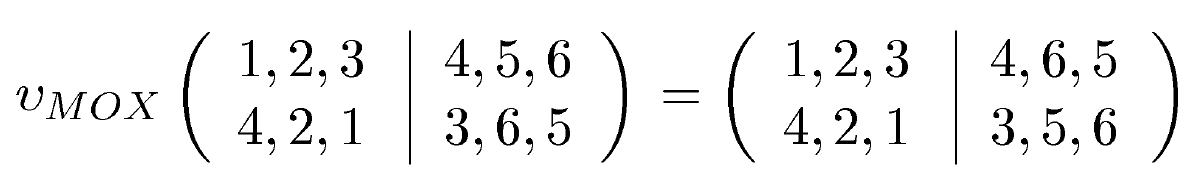
\includegraphics[width=0.9\textwidth]{Grafiki/MOX.png}
\end{center}
\end{spacing}
\end{frame}




\begin{frame}{RAND}
\begin{itemize}
\item Algorytm heurystyczno-losowy.
\item Zamiast algorytmu genetycznego używany jest losowy generator permutacji.
\end{itemize}

\end{frame}


\subsection{Porównanie wyników działania różnych wersji algorytmu}

\begin{frame}{Porównanie działania wersji algorytmu}
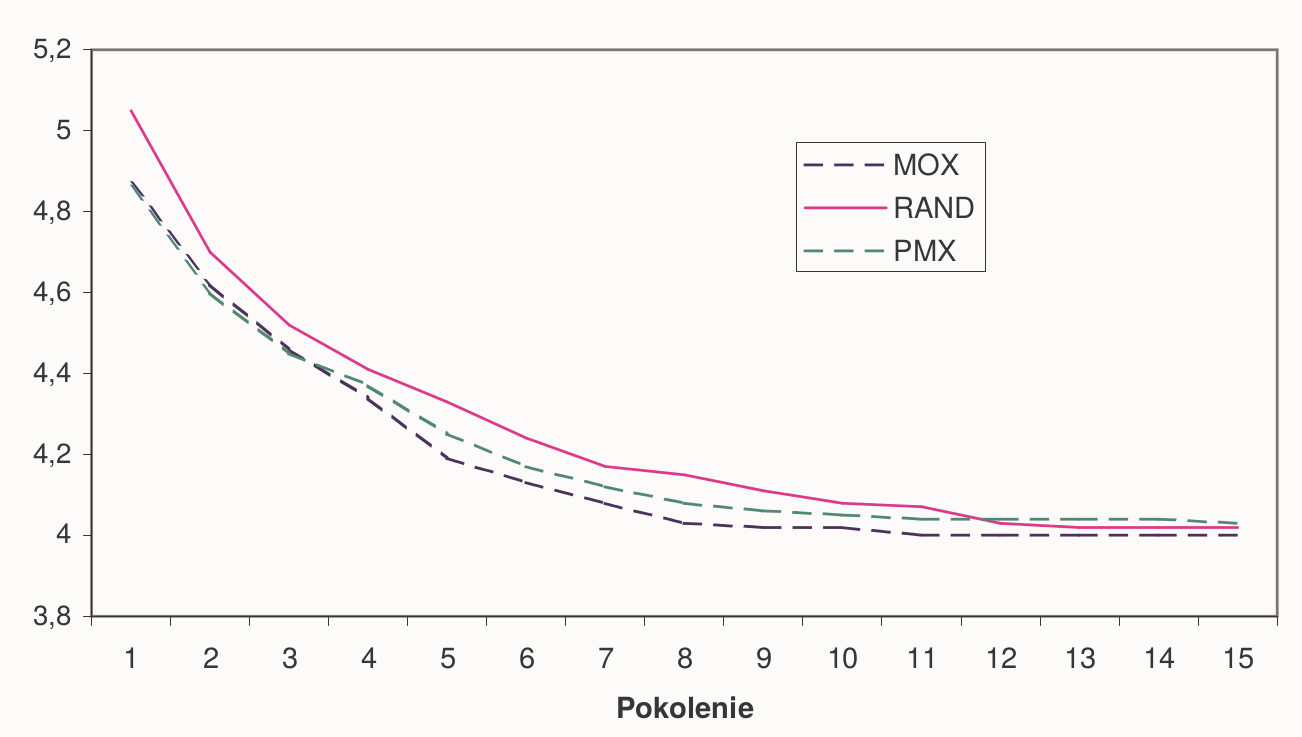
\includegraphics[width=1\textwidth]{Grafiki/wykresJW.png}
\end{frame}





% KONIEC – BIBLIOGRAFIA I SLAJD KOŃCOWY NA PYTANIA

\begin{frame}
\frametitle{Bibliografia}
\footnotesize
{
\begin{thebibliography}{99}
\bibitem{p1} Zdzisław Pawlak
\newblock Zbiory przybliżone -- nowa matematyczna metoda analizy danych 
\bibitem{p1} Leszek Rutkowski
\newblock Metody i techniki sztucznej inteligencji
\bibitem{p1} Lian Chen, Hongling Liu, Zilong Wan
\newblock An Attribute Reduction Algorithm Based on Rough Set Theory
and~an~Improved Genetic Algorithm
\bibitem{p1} Jakub Wróblewski
\newblock Adaptacyjne metody klasyfikacji obiektów
\end{thebibliography}
}
\end{frame}


{\1
\begin{frame}[plain,noframenumbering]
  \finalpage
  {
  \begin{huge}
  	Pytania
  \end{huge}
  
  }
\end{frame}
}

\end{document}